\documentclass[13pt,a4paper]{report}

\usepackage[T1]{fontenc}
\usepackage[romanian]{babel}
\usepackage{fontspec}
\usepackage[colorlinks]{hyperref}
\usepackage{graphicx}
\usepackage{wrapfig}

\addto\captionsromanian{\renewcommand{\abstractname}{Abstract}}

\begin{document}

\title{Money Stock}
\author{Barbu Paul - Gheorghe\\
Colegiul Național "Gheorghe Lazăr" - Sibiu\\
\texttt{paul.barbu@cnglsibiu.ro}}
\date{}
\maketitle

\begin{abstract}
Documentația programului Money Stock pentru Concursul de Informatică Aplicată
2012.
Acest program a fost creat plecând de la tema „Plus și Minus” având în vedere
fluctuațiile cursului valutar.
Aplicația este scrisă în C\# și folosește sursa on-line
\href{http://bnr.ro}{www.bnr.ro} pentru a
obține cursul valutar pentru monedele \\ disponibile.
\end{abstract}

\section{Scopul aplicației}
Scopul acestei aplicații este de a oferi utilizatorului o interfață simplă și
intuitivă pentru a putea schimba sume imaginare de bani în diferite monede.
Pe lângă funcționalitatea de bază, aplicația oferă posibilitatea de afișare a
cursurilor sub forma unui grafic, o metodă intuitivă pentru studierea evoluției
investițiilor.

\section{Seturile de date}
MoneyStock folosește cursurile valutare puse la dispoziție de BNR prin \\
intermediul fișierelor XML.
La fiecare pornire aplicația descarcă și parsează aceste feed-uri populând o bază
de date embedded.

Doar la prima pornire aplicația va descărca feed-ul din anul precedent \\ (calculat în
program), de exemplu
\href{http://bnr.ro/files/xml/years/nbrfxrates2011.xml}{feed-ul din anul 2011}, 
și va introduce aceste date în baza de date.

Apoi se vor prelua seturile de \href{http://bnr.ro/nbrfxrates10days.xml}{10
zile} și \href{http://bnr.ro/nbrfxrates.xml}{setul curent de date} lucru care se
va întâmpla la orice pornire ulterioară cu setul curent de date.
Setul de zece zile va fi preluat doar dacă datele locale sunt mai
vechi de zece zile.

\section{Baza de date}
Baza de date folosită este \texttt{Microsoft SQL Server Compact 3.5}, fiind una de
tip embedded nu necesită existența unui server, putând fi creată local pe orice
calculator.
Structura este integrată în program, tabelele fiind create dinamic în cod în
funcție de datele primite de la BNR.

Fiecare monedă are un tabel propriu după cum urmează:

\begin{center}
\begin{tabular}{| c | c |}
    \multicolumn{2}{ c }{nume monedă} \\ \hline
    rata de schimb & data cursului \\
    \hline
\end{tabular}
\end{center}

Cele două câmpuri reprezentând rata de schimb a monedei și data \\ 
calendaristică când aceasta e valabilă.

\section{Cursul valutar}
Principala funcționalitate oferită de Money Stock este cea de conversie a unor
sume de bani între monezi, aceasta oferind și posibilitatea adăugării TVA-ului la
suma curentă.
De asemenea este posibilă alegerea unei date calendaristice, caz în care ratele
de schimb se vor modifica reflectându-le pe cele de la data
selectată.

\begin{figure}[htb]
\centering
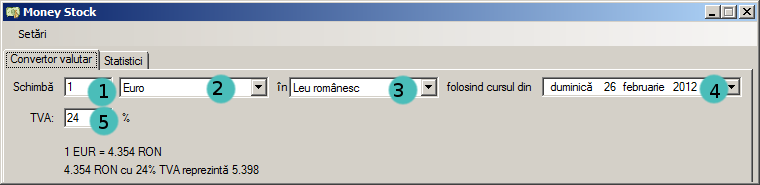
\includegraphics[width=1\textwidth]{img/ms.png}
\end{figure}

\begin{enumerate}
    \item Suma de schimb
    \item Moneda din care se schimbă
    \item Moneda în care se face schimbul
    \item Data la care schimbul are loc (influențează rata de schimb)
    \item Valoarea TVA-ului (în procente)
\end{enumerate}

\section{Statistică}
Când utilizatorul selectează tab-ul „Statistici” are posibilitatea de a vedea o
reprezentare a datelor sub formă de grafic.
Acest mod îi permite cu ușurință să facă comparații și să observe cum a evoluat
cursul valutar pe o perioadă de timp.

Perioada predefinită este de două săptămâni, iar monedele pre-selectate sunt
euro și dolarul american, acestea putând fi modificate cu ușurință.

Când pe grafic sunt reprezentate mai multe monede pe o perioadă lungă de timp,
acesta își pierde din acuratețe, acest lucru fiind contracarat de funcția
\texttt{zoom}.
Zoom-ul poate fi activat selectând cu click stânga o regiune a graficului
aceasta urmând să fie mărită și acuratețea reprezentării datelor să crească.

Pentru revenire la nivelul normal de zoom se poate da un click dreapta pe
grafic. Pentru a reveni un singur nivel de zoom trebuie folosit butonul 
care apare lângă barele de derulare.

\begin{figure}[htb]
\centering
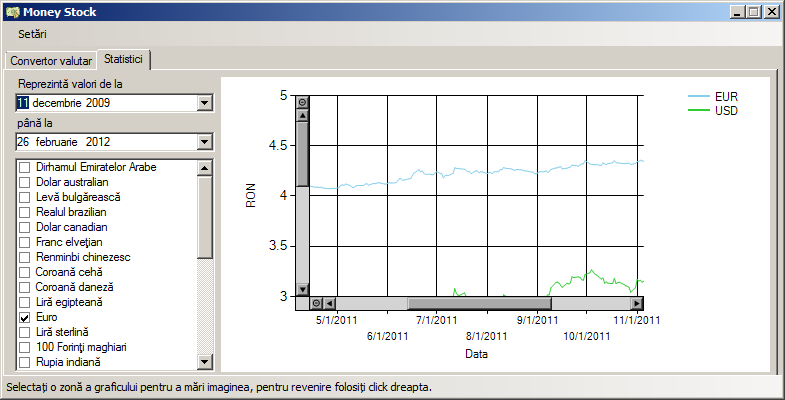
\includegraphics[width=1\textwidth]{img/zoom.png}
\end{figure}

\section{Funcții suplimentare}
Una dintre principalele funcții suplimentare este aceea că aplicația nu trebuie
repornită dacă ratele de schimb se modifică, actualizarea bazei de date fiind
posibilă din meniul „Setări”.

\begin{figure}[htb]
\centering
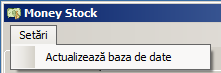
\includegraphics[scale=0.65]{img/settings.png}
\end{figure}

Atunci când nicio monedă nu e selectată în vederea reprezentării grafice,
aplicația își modifică automat forma evitând afișarea unui set de date gol.

\section{Validarea datelor}
În vederea rulării fără probleme când o sumă de bani este introdusă în
textbox orice caracter care nu ar putea forma un număr este automat șters,
evitând erorile legate de tipul de dată.

Luând în considerare faptul că ratele de schimb nu sunt cunoscute pentru viitor
toate obiectele \texttt{DateTimePicker} sunt restricționate până la data la care
se cunoaște un curs valutar.

Obținerea feed-urilor de date implică existența unei conexiuni active la
internet, în caz contrar baza de date nu se poate actualiza, apărând un mesaj de
eroare.

\begin{figure}[htb]
\centering
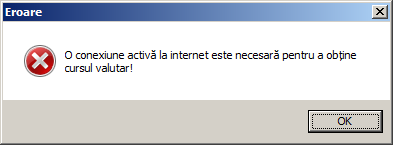
\includegraphics[scale=0.7]{img/error.png}
\end{figure}

\section{Cerințe}
Money Stock rulează nativ pe \texttt{.NET Framework 4.0}, nefiind necesare
biblioteci externe.
Dacă în schimb aplicația este rulată pe \texttt{.NET Framework 3.5} cele două
DLL-uri (incluse în arhiva programului) \texttt{System.Windows.Forms.DataVisualization.dll} 
și \texttt{System.Windows.Forms.DataVisualization.Design.dll} sunt necesare \\
deoarece \texttt{.NET 3.5} nu include suport nativ pentru grafice.

\end{document}
